Bei Nagios XI handelt es sich um eine webbasierte Anwendung. Die Software Nagios XI ist sowohl auf dem eigenen Server installierbar, als auch als SaaS. Die SaaS-L�sung ``Security Performance Availability Engine - SPAE'' die auf Nagios basiert, wird z.B. vom Unternehmen SHALB angeboten unter

\url{http://shalb.com/en/}

Im folgenden werden die Installationsschritte, die n�tig sind, um Nagios XI auf einem eigenen Server zu installieren, beschrieben. Die folgenden Schritte werden dabei auf einem Testrechner mit Ubuntu 12.04 ausgef�hrt.

Es wird die Free Trial Version von Nagios XI heruntergeladen unter:

\url{http://www.nagios.com/products/nagiosxi}

Die Trial Version ist eine 60 Tage Testversion von Nagios XI.

Es wird die VMware Virtual Machine (64-bit) Version 2012R1.6 heruntergeladen unter:

\url{http://library.nagios.com/library/products/nagiosxi/downloads/main}

Auf der viruellen Maschine ist Nagios XI 2012 und die Linux-Distribution CentOS 6.x vorinstalliert.

Um die VMware Virtual Machine starten zu k�nnen, muss VMware installiert werden. VMware kann kostenfrei heruntergeladen werden unter:

\url{https://my.vmware.com/web/vmware/free#desktop_end_user_computing/vmware_player/5_0}

Der heruntergeladene VMware-Player wird installiert mit:

\begin{verbatim}
sudo sh VMware-Player-5.0.1-894247.x86\_64.bundle
\end{verbatim}

Der VMware-Player wird gestartet und es wird die virtuelle Maschine ausgew�hlt mit ``Open a virtual Maschine''.

Die ausgew�hlte virtuelle Maschine wird gestartet mit ``play virtual maschine''.

Die virtuelle Maschine wird ausgef�hrt, d.h. CentOS wird gebootet und Nagios gestartet. In Abbildung \ref{fig:NagiosAufDerVirtuellenMaschine} auf Seite \pageref{fig:NagiosAufDerVirtuellenMaschine} ist Nagios auf der virtuellen Maschine zu sehen.

\begin{figure}[htp]
\centering
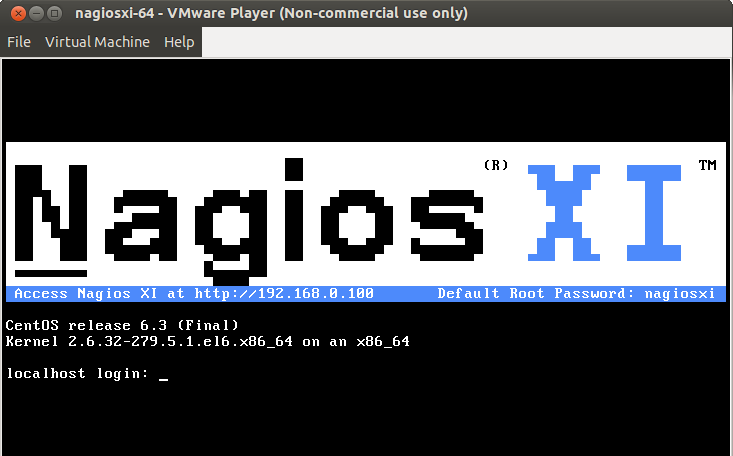
\includegraphics[width=0.6\textwidth]{ingo/bilder/virtuelleMaschine}
\caption{Nagios auf der virtuellen Maschine}
\label{fig:NagiosAufDerVirtuellenMaschine}
\end{figure}

Als n�chstes wird ein sicheres Kennwort vergeben. Damit kann auf Nagios XI �ber das Web Interface zugegriffen werden.

Dazu meldet man sich auf der virtuellen Maschine mit dem Root-Kennwort an.

\begin{verbatim}
Username: root
Password: nagiosxi
\end{verbatim}

Als n�chstes wird mit dem Befehl

\begin{verbatim}
passwd
\end{verbatim}

ein neues Root Kennwort vergeben. Im folgenden wird es auf 111sonoma222 ge�ndert.

Als n�chstes wird das MySQL Root Kennwort ge�ndert werden. Dazu wird der mysqladmin verwendet. Das Kennwort wird auf 111sonoma222 gesetzt

\begin{verbatim}
mysqladmin -u root -p'nagiosxi' password 111sonoma222
\end{verbatim}

Als n�chstes sollte das MySQL Backup Script angepasst werden. Es wird im Backup Script das neue Kennwort 111sonoma222 angegeben.
Das Backup Script wird mit folgendem Befehl editiert:

\begin{verbatim}
nano /root/scripts/automysqlbackup
\end{verbatim}

In diesem Script ist die Zeile 

\begin{verbatim}
PASSWORD=nagiosxi
\end{verbatim}

zu �ndern in

\begin{verbatim}
PASSWORD=111sonoma222
\end{verbatim}

Um die IP Adresse der virtuellen Maschine herauszufinden, wird folgender Befehl eingegeben:

\begin{verbatim}
ifconfig
\end{verbatim}

Hier steht unter eth0 $\rightarrow$ inet addr folgende IP-Adresse:

192.168.0.100

Mit dieser IP-Adresse kann auf des Web-Interface von Nagios XI zugegriffen werden.

In Abbildung \ref{fig:StartseiteVonNagios} auf Seite \pageref{fig:StartseiteVonNagios} ist die Starteseite von Nagios XI zu sehen.

\begin{figure}[htp]
\centering
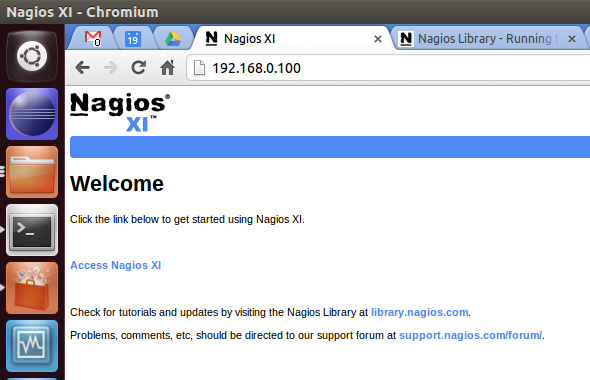
\includegraphics[width=0.6\textwidth]{ingo/bilder/Startseite}
\caption{Startseite von Nagios}
\label{fig:StartseiteVonNagios}
\end{figure}

Auf dem Web-Interface von Nagios kann auf Access Nagios XI geklickt werden, um Nagios XI einzustellen. Die Abbildung \ref{fig:NagiosXiEinstellen} auf Seite \pageref{fig:NagiosXiEinstellen} zeigt, dass an dieser Stelle folgende Punkte bearbeitet werden k�nnen:

\begin{itemize}
 \item die Prgramm URL, auf die die Nutzer auf Nagios zugreifen,
 \item der Administratorname,
 \item die EMail-Adresse des Administrators
 \item und das Administrator-Kennwort.
\end{itemize}

Nach einem Klick auf Install sollte die Installation von Nagios XI abgeschlossen sein.

\begin{figure}[htp]
\centering
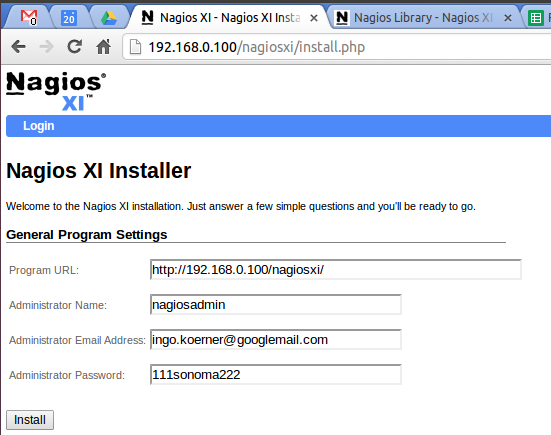
\includegraphics[width=0.6\textwidth]{ingo/bilder/NagiosInstall}
\caption{Nagios XI einstellen}
\label{fig:NagiosXiEinstellen}
\end{figure}

Leider kommt nach dem Klick auf Install eine Fehlermeldung. Diese Fehlermeldung ist in Abbildung \ref{fig:NagiosXiFehlermeldung} auf Seite \pageref{fig:NagiosXiFehlermeldung} zu sehen. Nach dem Klick auf Install kann nicht mehr auf das Web-Interface von Nagios XI zugegriffen werden.

\begin{figure}[htp]
\centering
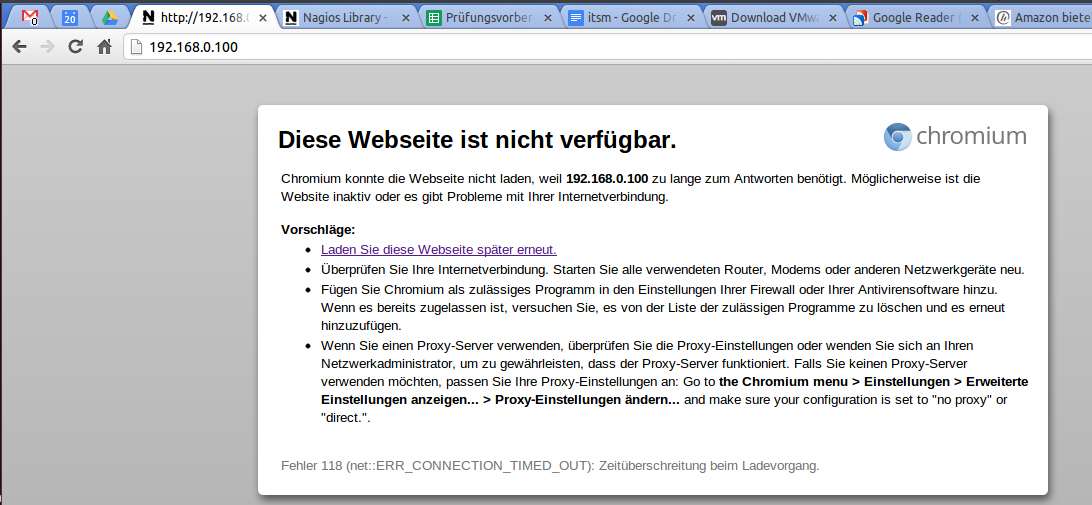
\includegraphics[width=0.6\textwidth]{ingo/bilder/NagiosFehler}
\caption{Nagios XI Fehlermeldung}
\label{fig:NagiosXiFehlermeldung}
\end{figure}

Der Zeitaufwand f�r die Installation von Nagios XI betr�gt ca. eine Stunde.

Die Software Nagios - dass damals noch NetSaint hie� - wurde 1999 von Ethan Galstad als Open Source Projekt in der Version Netsaint 0.0.1 ver�ffentlicht.
\url{http://www.nagios.org/about/history}
\url{http://www.ussrback.com/UNIX/audit/netsaint/index.html}

Es wird gesch�tzt, dass es weltweit ca 1 Million Nagios Nutzer gibt.
\url{http://www.nagios.org/about/community}

Nagios wird immernoch weiterentwickelt. Neue Releases sind geplant. Die letzte Version 2012R1.6 ist von 15. Februar 2013.